
\subsection{Setup}
\begin{figure}[H]
  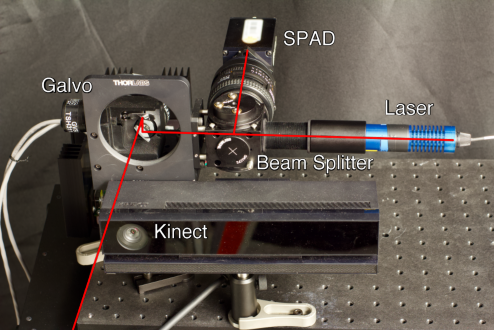
\includegraphics[width=\linewidth]{prototype_single_col.png}
  \caption{Prototype scanning setup. The pulsed light from the laser travels
    through a beam splitter before being guided by the galvo to the scene.
    Returning light is measured by the single-pixel SPAD. The RGB camera of a
    Kinect v2 is used to capture the monocular RGB image (the depth camera is
    not used)}
  \label{fig:prototype}
\end{figure}

